\subsection{Solstrålning genom fönster}

%Skapat med sunfigurestest
I figur \ref{fig:sun0415and1231} ses de relevanta vinklar som bildas av solens position den 15 april 2011 (heldragna linjer), samt den 31 december 2011 (streckade linjer), beräknat med funktionen sunposition i appendix \ref{sunposition}. Den röda linjen visar solens höjd över horisonten medan den gröna indikerar solens azimuthala vinkel, det vill säga vinkel i sidled från en referenspunkt, här tagen till ostlig riktning och positivt medsols. Slutligen representerar den blå linjen i figuren solens vinkel relativt en vertikal ytas normal (då denna pekar i horisontell sydlig riktning) och kan användas för att uppskatta effekten som solinstrålning bidrar till.

\begin{figure}[hpbt]
\centering
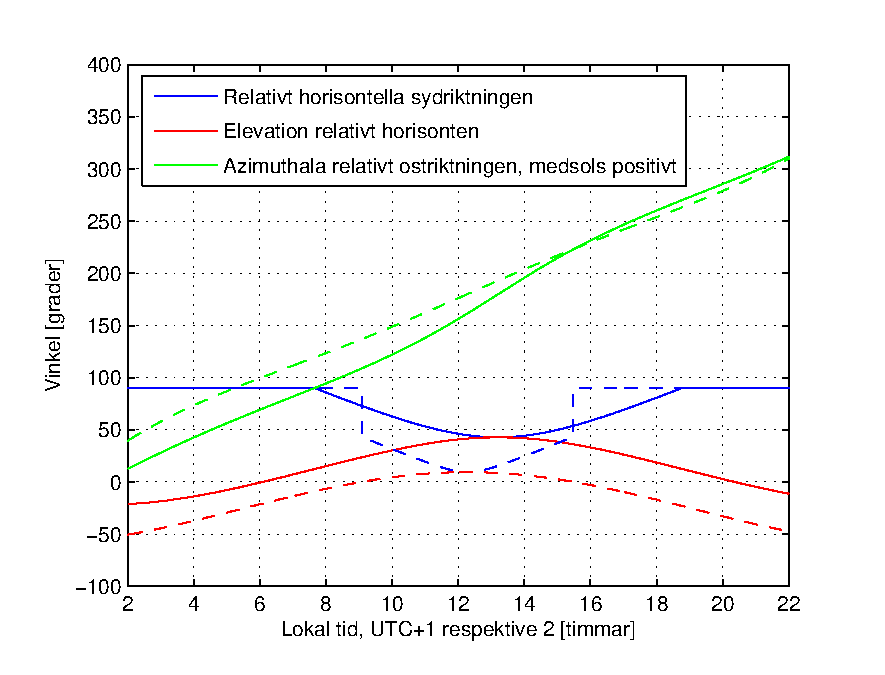
\includegraphics[scale=0.8]{images/sun0415and1231.eps}
\caption{\label{fig:sun0415and1231} Beräknade vinklar vid Walleriusgatan den 15 april 2011 (heldragna linjer, UTC+2) samt den 31 december samma år (streckade linjer, UTC+1).}
\end{figure}

Innan effekten beräknas måste dock ett exempel på solens intensitet över dagen skapas. % Teori om solintensitet över dagen?

Med denna intensitet, som kan ses i figur \ref{effekt0415and1231}, kan nu effektflödet beräknas.
Här antas fönstrets area uppgå till $\unit{1.5}{m^2}$,%AREA?
g-värdet för normal solstrålning är 0,45 % Referera till källan!
och konstanterna q och p i funktionen gvalue sätts till 4 respektive 3, ty fönstren i den avsedda byggnaden är av typ treglas utan ytbeläggningar.

% Figur här, för 110415 samt 111231, solintensitet och effekt utan gardiner och så.

%\begin{figure}[hpbt]
%\centering
%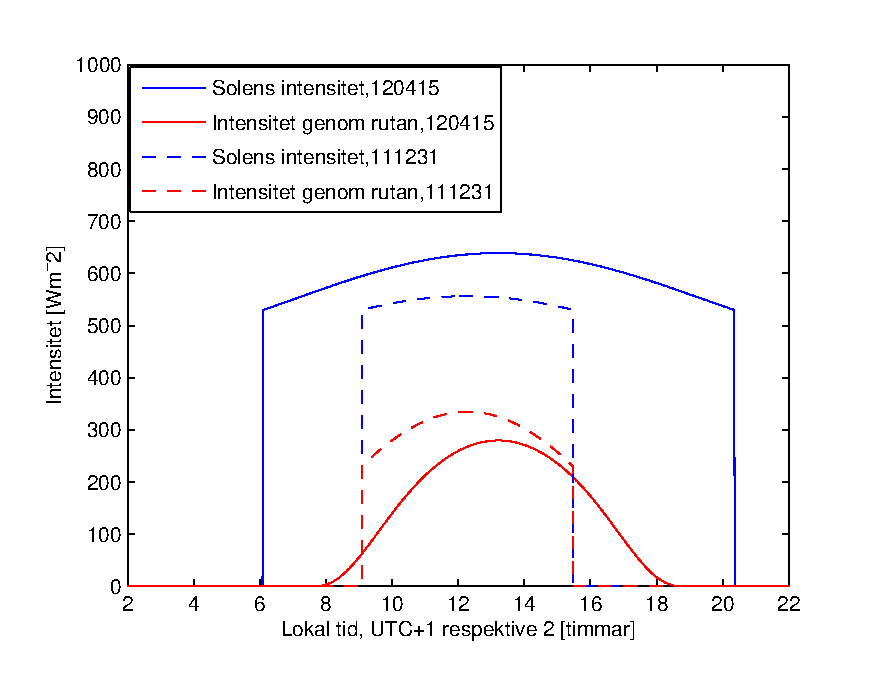
\includegraphics[scale=1]{images/effekt0415and1231.eps}
%\caption{\label{fig:effekt0101and0601} Beräknad effekt genom ett fönster vars normal pekar i horisontella sydriktningen, den första januari 2012 samt den första juni samma år. Solens intensitet varierar under dagen enligt den blå kurvan.}
%\end{figure}
